\documentclass[conference]{IEEEtran}

%%%%%%%%%%%%%%%%%%%%%%%%%%%%%
%%%%%%%% PACKAGES %%%%%%%%%%%
%%%%%%%%%%%%%%%%%%%%%%%%%%%%%
\usepackage{times}
\usepackage[numbers]{natbib}
\usepackage{multicol}
\usepackage[bookmarks=true]{hyperref}
\usepackage{amsmath}
\usepackage{amssymb}
\usepackage{graphicx}
\usepackage{caption}
\usepackage{stfloats} 

\begin{document}

\title{Sampling-Based and Contact-Implicit Nonprehensile \\ Manipulation using Signed Distance Functions}

% You will get a Paper-ID when submitting a PDF file to the conference system
\author{Author Names Omitted for Anonymous Review. Paper-ID [add your ID here]}

\author{
\authorblockN{Nikola Raicevic\authorrefmark{1},}
\authorblockA{\authorrefmark{1} Department of Electrical and\\Computer Engineering\\
University of California, San Diego\\
San Diego, California 92093-0013\\
Email: nmarinosraitsevits@ucsd.edu}
}

\maketitle
\IEEEpeerreviewmaketitle

\newpage
\section{Page Break}
\newpage
\section{Page Break}
\newpage

\begin{figure*}[!t]
  \centering
  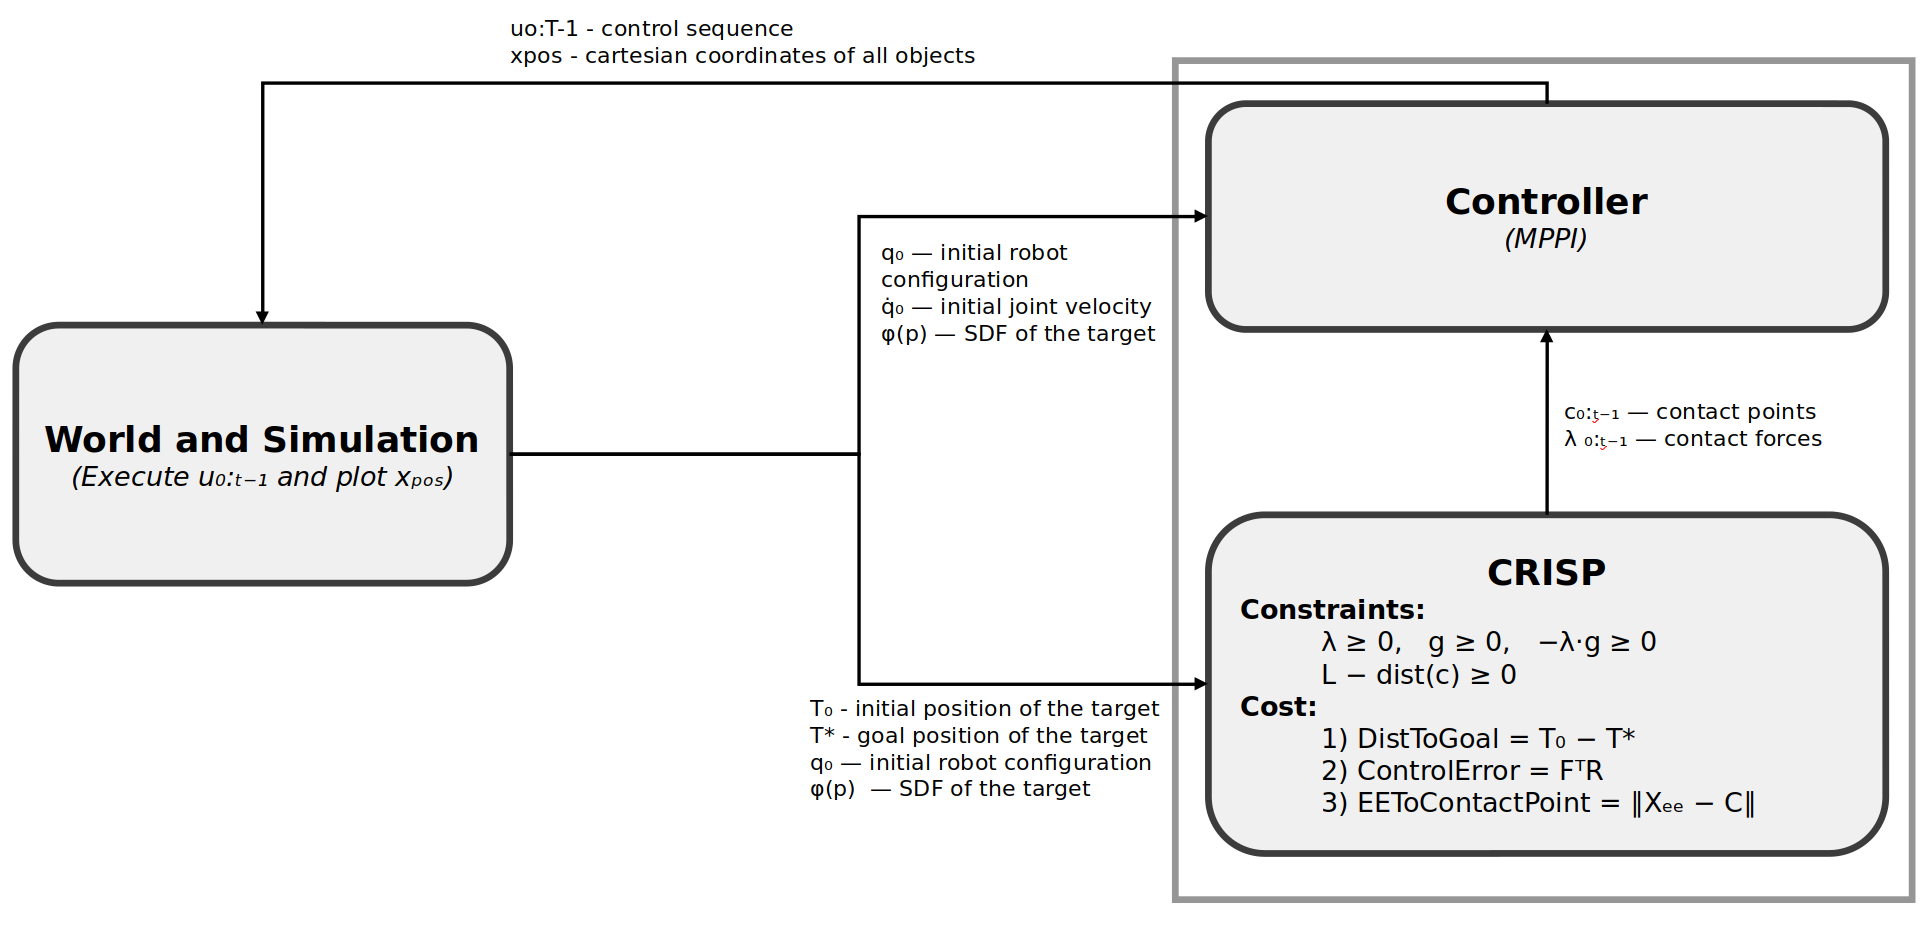
\includegraphics[width=\textwidth]{Figs/Chart.png}
  \caption{Contact-implicit motion using signed distance functions and diffusion-inspired annealing control.}
  \label{fig:contact-implicit-motion}
\end{figure*}

%=============================
% Problem Formulation
%=============================
\section{Problem Formulation}
\noindent\textbf{Objective:} Given a robot's initial configuration $q_0$ and the signed distance function of the target object $\phi(p)$, find a sequence of controls $\{u_0, u_1, \dots, u_{T-1}\}$ to relocate an object from start pose $T_0\!\in\!SE(2)$ to goal pose $T^*\!\in\!SE(2)$ while respecting unilateral contact and friction.
\medskip

\textbf{Given:}
\begin{itemize}
    \item $T_0$ — Initial object pose
    \item $T^*$ — Goal object pose
    \item $q_0$ — Initial robot configuration
    \item $u_{0}$ — Initial robot controls (i.e. velocities,torques)
    \item $\phi(p)$ — Signed distance function (SDF) of the target  
\end{itemize}

\medskip
\noindent The system architecture consists of a simulator environment that provides the initial state variables $(T_0, T^*, q_0, u_0)$ and access to the signed distance functions $\phi(p)$. These inputs are processed by the \textbf{CRISP} module and a motion controller. The CRISP module defines an object-centric policy:
\[
\pi(T_0, T^*, q_0, \phi(p)) = (c, F)
\]
which solves an optimization problem to generate a contact trajectory $\{c_0, \dots, c_{T-1}\}$ and a sequence of contact forces $\{\lambda_0, \dots, \lambda_{T-1}\}$. These are then passed to a controller that constructs a reward function guiding the manipulator to the desired contact points to push or reposition the target object.

The controller performs trajectory rollouts and returns the control sequence $\{u_0, \dots, u_{T-1}\}$ and the predicted Cartesian object positions $x_{\text{pos}}$. These trajectories are then fed back into the simulator for visualization and validation.
\newpage

%=============================
% Object Modeling
%=============================
\section{Object Modeling}
\noindent We optimize the pose trajectory $x_{0:T}$ and controls $u_{0:T}$
\[
x_t=\begin{bmatrix}p_{x,t}&p_{y,t}&\theta_t\end{bmatrix}^\top\qquad
u_t=\begin{bmatrix} c_t\\ \lambda_t\end{bmatrix}
\]
where $c_t\!\in\!\mathbb{R}^2$ is the contact location (in the body frame), $p\!\in\!\mathbb{R}^2$ is the position of the target, $\theta\!\in\!\mathbb{R}$ is the orientation of the target, and $\lambda_t$ are the force parameters of the selected model (Sec.~\ref{subsec:crisp-models}). Each method defines associated inequality constraints ensuring unilateral contact and friction consistency plus a differentiable map:
\[
\mathcal{F}_\mathsf M:\;(x_t, c_t, \lambda)\;\mapsto\; \big( F^w_t,\tau_t\big),
\]
where $\mathsf M\in\{\text{M1},\text{M2},\text{M3},\text{M4}\}$ selects the force model
\medskip

% Object Kinematics
\subsection{Object Kinematics}
\noindent We separate \emph{kinematics} (how pose evolves) from \emph{wrench generation} (how contact forces/torques arise). Explicit-Euler kinematics equation:
\[
g^{dyn}_t(x_t,u_t)=
\begin{bmatrix}
     p_{t+1}- p_t-\Delta t\,v_t\\[0.15em]
    \theta_{t+1}-\theta_t-\Delta t\,\omega_t
\end{bmatrix}= 0, \quad
\dot{{p}}_t = {v}_t\quad
\dot{\theta}_t = \omega_t
\]
where $\Delta t$ is an Euler discretization time-step. This model is appropriate when inertia is non-negligible.
\medskip

% Object Dynamics
\subsection{Object Dynamics (Quasi-Static Model)}
\noindent We assume a quasi-static regime: inertial terms are negligible and the resistive ground wrench balances the applied contact wrench at each step. 
\[
\sum^N_{i=0} F_{i} = 0 => F_{c} = F_{f} = \mu vF_{N}
\]
With normal load \(mg\) and isotropic Coulomb friction \(\mu\), we use a diagonal mobility model that maps the world wrench to the body twist:
\[
\begin{bmatrix} v_{x,t} \\[0.2em] v_{y,t} \\[0.2em] \omega_t\end{bmatrix}
=\frac{1}{\mu m g}
\begin{bmatrix}
F^w_{x,t} \\[0.2em] F^w_{y,t} \\[0.2em] (\tau_t \cdot m)/I_{z}
\end{bmatrix},
\quad I_{z}=\tfrac{1}{12}m\sqrt{a^2+b^2} \quad(\text{box})
\]

\noindent where \(a,b\) are the half-sizes of the rectangles, ${F}^w_t\in\mathbb{R}^2$ is the force of the world frame, $\tau_t\in\mathbb{R}$ is the torque about the COM and \(I_{z}\) is the moment of inertia. The world-frame force is \( F^w_t=R(\theta_t)\, F^b_t\) where $R(\theta_t)$ maps body $\{b\}$ to world $\{w\}$ with 
\[
R(\theta)=\begin{bmatrix}\cos\theta&-\sin\theta\\ \sin\theta&\cos\theta\end{bmatrix}
\]
Moments about the COM use the 2-D cross product of the lever arm and the body-frame force:
\[
\tau_t = c_{x,t} F^b_{y,t} - c_{y,t} F^b_{x,t}
\]
\newpage

%=============================
% CRISP
%=============================
\section{CRISP}
\noindent We consider planar, contact-rich manipulation (e.g., pushing) where an object with a pose $\;x_t = [\,p_{x,t},\,p_{y,t},\,\theta_t\,]^\top\,\in \mathbb{R}^3$ is driven toward a goal by applying contact force subject to frictional constraints. The key difficulty is that both \emph{where} to push (contact point(s) $\mathbf{c}_t\in \mathbb{R}^2$) and \emph{how} to push (contact force(s) $\boldsymbol{\lambda}_t$) must be chosen so that: \newline
(i) the object moves as desired; \newline
(ii) contact remains feasible (unilateral contact and friction). \newline
(iii) The model remains differentiable for gradient-based optimization. \newline

\noindent CRISP casts this as a smooth trajectory optimization problem over $\{x_t,u_t\}_{t=0}^{T}$ with differentiable dynamics and contact models, enabling gradient-based solvers to optimize states and controls under equality/inequality constraints jointly. In our implementation, we use two \emph{wrench-generation} models: \newline
(i) An analytical, face-aligned model tailored to rectangular objects. \newline
(ii) A geometry-agnostic signed-distance function (SDF) normal model for arbitrary shapes.
Both produce a body/world-frame wrench that feeds the dynamics and constraints.

% Merit Function
\subsection{Merit Function and Exact-Penalty Form}
\noindent We use a composite exact penalty to trade off objective decrease and constraint violation:
\begin{equation}
\label{eq:merit}
\varphi(x;\mu)=J(x)+\!\!\sum_{i\in\mathcal E}\!\mu_i\,\big|g_i(x)\big|
+\!\!\sum_{j\in\mathcal I}\!\mu_j\,\big[g_j(x)\big]^{-},
\; [a]^{-}=\max\{0,-a\}
\end{equation}
where $J$ collects stage costs and $g=(g^{\text{dyn}},g^{\text{equality}},g^{\text{inequality}})$ stacks equalities and inequalities. 

% SQP Subproblem with TR
\subsection{SQP Subproblem with Trust Region}
\noindent At iterate $x^{(k)}$, we build a local quadratic model of $J$ and linearize constraints:
\begin{equation}
\label{eq:sqp}
\begin{aligned}
\min_{p_k}\; \underbrace{J_k+\nabla J_k^\top p_k+\tfrac12 p_k^\top \nabla^2_{xx}J_k\,p_k}_{\text{quadratic model of }J}
+\!\!\sum_{i\in\mathcal E}\!\mu_i\big|g_i(x_k)+\nabla g_i(x_k)^\top p_k\big| \\
+\!\!\sum_{i\in\mathcal I}\!\mu_i\,[g_i(x_k)+\nabla g_i(x_k)^\top p_k]^{-} \\
\text{s.t.}\quad f(x_k)+\nabla f(x_k)\,p_k=0,\qquad \|p_k\|\le \Delta^{(k)}
\end{aligned}
\end{equation}
where $f$ stacks the equality constraints (e.g., dynamics defects) and $J_k,\nabla J_k,\nabla^2_{xx}J_k$ evaluated at $x_k$. The radius of the trust region $\Delta^{(k)}$ controls the non-linearity.

\paragraph{Step acceptance.}
Let $m^{(k)}(p)$ be the local model of $\varphi$. Define
\[
\begin{aligned}
\mathrm{pred} &= \varphi(x^{(k)};\mu) - m^{(k)}(p) \\
\mathrm{ared} &= \varphi(x^{(k)};\mu) - \varphi(x^{(k)}\!+\!p;\mu) \\
\rho &= \frac{\mathrm{ared}}{\mathrm{pred}}
\end{aligned}
\]

Accept if $\rho\ge \eta$ and update the radius
\[
\Delta^{(k+1)}=
\begin{cases}
\gamma_{\uparrow}\Delta^{(k)},& \rho\ \text{large}\\
\gamma_{\downarrow}\Delta^{(k)},& \rho\ \text{small}\\
\Delta^{(k)},& \text{otherwise.}
\end{cases}
\]

\paragraph{Penalty updates and stopping}
Increase $\mu_i$ for stalled violations (cap at $\mu_{\max}$); stop when (i) the merit decrease is small and (ii) equality/inequality violations and KKT residuals fall below tolerances.

% Algorithm
\subsection{Algorithm}
\label{subsec:crisp-algo}
\begin{minipage}{0.98\linewidth}
\begin{enumerate}\itemsep3pt
\item Initialize $(x^{(0)},\mu^{(0)},\Delta^{(0)})$ and choose a wrench model $\mathsf M$.
\item Repeat ($k=0,1,\dots$) until convergence:
  \begin{enumerate}\itemsep2pt
  \item Linearize $f,g$ at $x^{(k)}$; form $J^{(k)}$ build trust-region SQP.
  \item Handle complementarity via penalties in $\phi$.
  \item Solve the TR-SQP subproblem~\eqref{eq:sqp} to get step $p^{(k)}$.
  \item Compute $\rho$ (predicted vs.\ actual merit decrease) and accept/reject; update $\Delta$ by shrink/expand trust region.
  \item Update penalties $\mu$ (bounded by $\mu_{\max}$) if constraints stall. For violated constraints $\mu$ $\uparrow$.
  \item Check convergence: merit decrease + constraint violation/KKT residual below tolerance.
  \end{enumerate}
\end{enumerate}
\end{minipage}

% CRISP Objective Function
\subsection{Objective Function}
\noindent Minimize the cost of tracing the pose at $T^\star$ with small force penalties and contact wandering, subject to dynamics, boundary/SDF, and friction constraints.
\medskip

\noindent\textbf{Objective:}
\begin{align*}
\min_{\{x_t, c_t,z_t\}} \quad
    \underbrace{\ell_T(x_T;T^\star)}_{\text{terminal pose track}} 
    + \sum_{t=0}^{T-1} \Big(\underbrace{\ell_x(x_t;T^\star)}_{\text{running track}}
    + \underbrace{\ell_c( c_{t+1}- c_t)}_{\text{contact TV}} \\
    + \underbrace{\ell_z(z_t)}_{\text{force reg.}}\Big)
\end{align*}
Where quadratic costs with weights: strong terminal $Q$, weak running $P$, small $\ell_2$ on forces $R$, and medium on contact points $M$. Terminal quadratic tracking on \((p_x,p_y,\theta)\), total-variation on \(c_t\), and quadratic penalties on \(\lambda_t\).
\medskip

% CRISP Constraints
\subsection{Equality and Inequality Constraints}
\label{subsec:crisp-constraints}

\noindent
CRISP enforces \emph{two} kinds of constraints:
(i) equality constraints that come \emph{solely} from the discretized dynamics, and
(ii) inequality constraints that encode contact admissibility and friction, which are
\emph{model-specific} (see Sec.~\ref{subsec:crisp-models}).

\paragraph{Equality constraints (from dynamics), $t=0{:}T-1$}
\[
\begin{aligned}
 p_{t+1}- p_t-\Delta t\,v_t &=  0, 
\qquad
\theta_{t+1}-\theta_t-\Delta t\,\omega_t = 0,
\end{aligned}
\]
where $(v_t,\omega_t)$ are obtained from the chosen mobility law
(quasi-static or Newtonian) given the method’s wrench $( F^w_t,\tau_t)$.

\paragraph{Inequality constraints (contact model)}
These depend on the selected model $\mathsf M \in \{\text{M1},\text{M2},\text{M3},\text{M4}\}$ in Sec.~\ref{subsec:crisp-models}:
\begin{itemize}
\item \textbf{Contact location admissibility (boundary/SDF).}
The contact point must lie on the object boundary. With a body-frame SDF $\phi$,
\[
\phi( c_t)=0 \quad \text{(exact or softened).}
\]
For rectangles (half-sizes $a,b$) an equivalent boundary form is
\(\max(|c_{x,t}|-a,\;|c_{y,t}|-b)=0\) (often implemented softly).

\item \textbf{Unilateral contact and friction.}
Each model imposes its own feasible set:
\[
\text{e.g.,}\quad
\lambda_t \ge 0,\qquad
\| f_{t,\mathrm{tang}}\|_2 \le \mu\,f_{t,\mathrm n}
\quad\text{(M2/M3),}
\]
or a \emph{limit-surface} bound on the planar wrench
\( w_t=[F^w_{x,t},F^w_{y,t},\tau_t]^\top\) (M1/M3),
or an $\ell_\infty$ box surrogate on forces/torque (M4).
The exact inequalities are specified per model in Sec.~\ref{subsec:crisp-models}.
\end{itemize}

\paragraph{Complementarity and smoothing.}
Single-contact exclusivity and non-penetration $\perp$ normal-force are handled via smooth surrogates
(e.g., product terms, soft-abs/max) embedded in the inequality set, and are weighted in the
\emph{exact-penalty} merit function \(\varphi(\cdot;\mu)\) in~\eqref{eq:merit}.
This keeps the overall program differentiable for the SQP/trust-region solver.

% CRISP Models
\subsection{CRISP Models}
\label{subsec:crisp-models}
\noindent We \emph{share} the dynamics across methods and only swap the wrench map and inequalities:

% M1
\subsubsection{(M1) Four face-aligned forces (rectangle)}
For the analytical model we use $\boldsymbol{\lambda}_t\in\mathbb{R}^4$ (one scalar per face direction).
\begin{align}
\mathbf F^{b}_t &=
\begin{bmatrix}
\lambda_{2,t} + \lambda_{4,t} \\
\lambda_{1,t} + \lambda_{3,t}
\end{bmatrix},\;
\tau_t = c_{x,t}\,(\lambda_{1,t}+\lambda_{3,t}) - c_{y,t}\,(\lambda_{2,t}+\lambda_{4,t}) \label{eq:m1_force}
\end{align}

\[
\text{where}\; \lambda_t = [\lambda_{1,t},\lambda_{2,t},\lambda_{3,t},\lambda_{4,t}]^\top\in\mathbb{R}_{\ge 0}^4,
\]
One nonnegative scalar per face (bottom/left/top/right) in body frame. We assemble a body-frame net force consistent with face directions and set \(\mathbf F^w_t = R(\theta_t)\,\mathbf F^b_t\). \\
\textbf{Inequalities:}
\[
\lambda_{i,t}\ge 0\quad \forall i,
\quad
\underbrace{\max(|c_{x,t}|-a,\;|c_{y,t}|-b)}_{\text{on boundary}}=0,
\]

Enforce \emph{single-contact exclusivity} via smooth products:
\[
\lambda_{i,t}\lambda_{j,t}\le 0\;(i\neq j)\quad\quad \text{(complementarity surrogate)}
\]

% M2
\subsubsection{(M2) One resultant force} single resultant (normal-only $\lambda_t$ or free $ F^b_t$) with one cone. \\
\textbf{Inequalities:}
\[
\lambda_{t}\ge 0\quad,
\quad
\]

% M3
\subsubsection{(M3) $\ell_\infty$ surrogate:} $\ell_\infty$ surrogate (box) for friction/limit-surface.
\[
\lambda_{t}\ge 0\quad,
\quad
\]

% M4
\subsubsection{(M4) SDF-normal} for the SDF model we use a single normal load $\lambda_t\in\mathbb{R}_{\ge 0}$.
\[
F^b_t=\lambda_t\, n^b( c_t), \; \tau_t=(c_x n_y^b-c_y n_x^b)\lambda_t \quad \text{where} \;   n^b( c_t) = -\frac{\nabla\phi( c_t)}{\|\nabla\phi( c_t)\|}
\]
\textbf{Inequalities:}
\[
\phi( c_t)\ge0, \quad \lambda_t \in \mathbb{R}_{\ge 0}
\]

\subsection{Implementation Notes and Code Mapping}
\label{subsec:impl-mapping}
Our C++ setup mirrors this formulation:
\begin{itemize}
\item \textit{Dynamics equalities:} \\
\texttt{pushboxDynamicConstraints} implements dynamics with explicit Euler.

\item \textit{Contact/friction inequalities:} \\
\texttt{pushboxContactConstraints} encode boundary, unilateral, and friction (smoothed); \texttt{pushboxContactSingleForceConstraints} adds single-contact exclusivity via smooth products.

\item \textit{Objective:}\\
\texttt{pushboxObjective} uses strong terminal tracking ($Q$), weak running tracking ($P$), TV-like smoothing on $\mathbf c_t$ ($M$), and small $\ell_2$ on forces ($R$).

\item \textit{TR+penalty hyperparameters:} \\
are set via \texttt{muMax}, \texttt{trailTol}, \texttt{trustRegionTol}, \texttt{constraintTol}, \texttt{WeightedMode}, \texttt{WeightedTolFactor}, matching the updates in Sec.~\ref{subsec:crisp-algo}
\end{itemize}













\newpage
\section{Page Break}
\newpage
\section{Page Break}
\newpage
\section{Page Break}
\newpage

%%%%%%%%%%%%%%%%%%%%%%%%%%%%%
%%%%%%%% ABSTRACT %%%%%%%%%%%
%%%%%%%%%%%%%%%%%%%%%%%%%%%%%
\begin{abstract}
We demonstrate the integration of environment information, represented as a Signed Distance Function (SDF), into a contact-implicit motion planning and control framework. Building upon the Diffusion-Inspired Annealing for Legged MPC (DIAL-MPC) paradigm—a sampling-based Model Predictive Control (MPC) method that leverages a diffusion-style annealing process—we design a reward function centered on the SDF value and its gradient. This allows the controller to estimate both the distance to the contact surface and the direction of force application, enabling more informed and robust contact reasoning. Furthermore, we model discrete target locations probabilistically through the SDF, which enables the controller to reason over uncertainty in target observations. To the best of our knowledge, this is the first demonstration of using SDFs within an MPC framework to formulate a reward function for contact-implicit motion. Our approach showcases how structured environment representations can enhance the expressiveness and effectiveness of parallelized planning and control pipelines.
\end{abstract}

%%%%%%%%%%%%%%%%%%%%%%%%%%%%%
%%%%%% INTRODUCTION %%%%%%%%%
%%%%%%%%%%%%%%%%%%%%%%%%%%%%%
\section{Introduction}
Robotic manipulators have demonstrated impressive capabilities in complex environments using traditional motion planning algorithms. However, these approaches often struggle in dynamic or contact-rich settings where re-planning must occur frequently due to changes in the environment. In such scenarios, high-level motion planning is typically augmented with low-level controllers that track local trajectories. Yet, contact-rich tasks pose significant challenges for both motion planning and control due to the non-smooth, hybrid nature of multi-contact dynamics, which are often modeled through complementarity constraints. These models introduce combinatorial complexity and non-convexity, rendering real-time optimization in high-dimensional spaces intractable for many classical planning methods.

Recent advances in sampling-based Model Predictive Control (MPC) offer a promising alternative. In particular, Diffusion-Inspired Annealing for Legged MPC (DIAL-MPC) \cite{xue2024fullordersamplingbasedmpctorquelevel} enables efficient online optimization by sampling and refining control sequences through a diffusion-style annealing process. DIAL-MPC achieves global exploration and local convergence, making it well-suited for high-dimensional manipulators where exhaustive search is infeasible. This approach leverages the massive parallelization capabilities of MuJoCo to simulate thousands of rollouts in parallel, allowing the reward function to effectively guide control sequence selection at each timestep.

Simulation-to-reality transfer has also shown strong potential in contact-rich control. For example, whole-body control on quadruped and humanoid robots has been demonstrated using iterative Linear Quadratic Regulator (iLQR) methods \cite{zhang2025wholebodymodelpredictivecontrollegged}, where MuJoCo-based simulation and finite-difference derivatives are used to design controllers with minimal real-world fine-tuning.

Model Predictive Path Integral (MPPI) controllers further extend the benefits of parallelization by using GPU-accelerated physics simulators such as IsaacGym to evaluate the rollout costs of thousands of candidate trajectories in real-time \cite{pezzato2025samplingbasedmodelpredictivecontrol}.

Reinforcement learning (RL)-based approaches have also been applied to contact-rich manipulation, where policies are trained in latent or task-specific representations to solve tasks such as picking, lifting, and stacking \cite{hansen2024tdmpc2scalablerobustworld}. However, these methods are often data-intensive and struggle to generalize to high-dimensional manipulators, where collecting sufficient training data becomes impractical.

Several hybrid approaches attempt to bridge the gap between analytical modeling and learning. For instance, adaptive contact-implicit MPC methods combine prior model knowledge with online residual learning to compensate for modeling errors \cite{huang2024adaptivecontactimplicitmodelpredictive}. These methods improve robustness to modeling inaccuracies but still require significant offline tuning or high-quality priors.

Alternatively, physics-informed modeling approaches aim to sidestep the computational challenges of complementarity-based contact models. Recent work has demonstrated complementarity-free multi-contact modeling, achieving faster and more reliable optimization for dexterous manipulation tasks by reformulating the contact dynamics \cite{jin2025complementarityfreemulticontactmodelingoptimization}.

In this work, we extend the DIAL-MPC framework by incorporating structured environment information in the form of a Signed Distance Function (SDF). This enables contact-implicit control where surface geometry and proximity are directly encoded in the reward function. By leveraging SDF values and gradients, the controller gains insight into both the distance to the contact surface and the direction of force application. Additionally, we formulate discrete target locations probabilistically via the SDF, enabling more robust reasoning over uncertainty in target observations. To our knowledge, this is the first instance of integrating SDF-based reward shaping into a sampling-based MPC framework for contact-implicit manipulation.

%%%%%%%%%%%%%%%%%%%%%%%%%%%%%
%%%%%% RELATED WORK %%%%%%%%%
%%%%%%%%%%%%%%%%%%%%%%%%%%%%%
\section{Related Work}

\subsection{Sampling-Based Model Predictive Control}

Sampling-based MPC methods have emerged as powerful tools for high-dimensional, nonlinear control. Algorithms such as MPPI \cite{pezzato2025samplingbasedmodelpredictivecontrol} and DIAL-MPC \cite{xue2024fullordersamplingbasedmpctorquelevel} exploit parallelized simulation to evaluate control rollouts and optimize trajectories in real-time. These methods are particularly suited for complex manipulation tasks, where gradient-based solvers may fail due to non-smooth cost landscapes or contact discontinuities. By drawing samples from a policy distribution and refining them iteratively, these controllers achieve a balance between global exploration and local exploitation.

\subsection{Contact-Implicit Motion and MPC}

Traditional contact-implicit methods rely on complementarity constraints to model multi-contact interactions. These formulations, while physically grounded, introduce significant computational overhead due to their non-convex and hybrid nature. Recent methods have sought to overcome this by using learning-based residual models \cite{huang2024adaptivecontactimplicitmodelpredictive} or reformulating the contact model entirely \cite{jin2025complementarityfreemulticontactmodelingoptimization}. In contrast, our approach leverages SDFs as a lightweight and differentiable proxy for contact geometry, enabling efficient reward shaping without the burden of hybrid dynamics solvers.

\subsection{Environment-Aware Control and SDF Representations}

Signed Distance Functions are commonly used in robot perception and mapping, but their integration into control pipelines remains underexplored. Recent works have demonstrated the utility of SDFs in perception-aware planning and model-based RL, particularly for encoding implicit shape priors. Our work uniquely integrates SDFs into a sampling-based MPC controller to encode both contact geometry and probabilistic target distributions, enabling real-time, contact-aware control without explicit collision modeling.


%%%%%%%%%%%%%%%%%%%%%%%%%%%%%
%%%%%%%% METHOD %%%%%%%%%%%
%%%%%%%%%%%%%%%%%%%%%%%%%%%%%
\section{Technical Approach}

\section{Preliminary}
% Dial MPC - Key equations 


\section{Cost-Function Design}
% Contact point and the gradient: add the visualization (configuration of the robot, how we compute the reward function)



%%%%%%%%%%%%%%%%%%%%%%%%%%%%%
%%% RESULTS & EVALUATION %%%%
%%%%%%%%%%%%%%%%%%%%%%%%%%%%%
\section{Results $\&$ Evaluation}





%%%%%%%%%%%%%%%%%%%%%%%%%%%%%
%%%%%%% CONCLUSION %%%%%%%%%%
%%%%%%%%%%%%%%%%%%%%%%%%%%%%%
\section{Conclusion} 
\label{sec:conclusion}
The conclusion goes here.


\section*{Acknowledgments}


%% Use plainnat to work nicely with natbib. 
\bibliographystyle{plainnat}
\bibliography{references}



\section{Requirements} 
What to Submit? Each submitted Demo paper will include a manuscript describing the system (see format and length recommendations below) and demonstrations of the system itself, which can be accessed by reviewers via the supplementary material (e.g., executable software, multimedia showing the operation of robotic hardware, demonstrations of the achieved scalability, etc.), or via a link to a website that is accessible at the time of the review period.

Single-blind: Demo paper submissions are allowed (but not required) to be single-blind in contrast to Science/System papers, which must be double-blind. Demo paper submissions are understood to be demonstrating unique systems that will obviously reveal the authors or their affiliations. Demo papers are not opportunities to bypass the double-blind requirement of Science/System submissions. The reviewers will be asked to evaluate whether a submission was appropriately submitted under the Demo paper category.

Submission Requirements: The authors of Demo paper submissions are required to start the title of the submission with the word “Demonstrating” to communicate to the reviewers the type of submission and that they are allowed to be single-blind. The authors of Demo papers are also asked to include a short 1-paragraph section at the time of the submission titled “Intended Demonstration” (e.g., before or after the introduction section of their submitted manuscript), of how they envision that the RSS live audience will experience the demonstrated system. See examples of ways to demonstrate a system below. This section can be removed at the time of the Camera-Ready submission, if the Demo paper is accepted.

\section{Topics}
Link: https://sites.google.com/rice.edu/parallelized-planning-control/

We invite paper submissions on various aspects of motion planning and control via parallelization, including but not limited to the following topics:

    How can parallelism improve sampling-based, search-based, optimization-based and learning-based motion planning?

    How can parallelism improve robot control, e.g., model predictive control (MPC) techniques?

    How can one account for nonlinear constraints such as robot dynamics, contact dynamics, state space manifolds, etc. with parallelization techniques?

    What environment representations are compatible with parallelized motion planning and control?

    What are the new roles of planning and control in robot autonomy, as parallelized motion planning can achieve microseconds to milliseconds planning time?

As a non-archival workshop, we also welcome recent published or submitted results on the relevant topics. The submissions will be reviewed, and if accepted, will be posted on the workshop website and presented at our poster session.

\subsection{RSS Hyperlinks}

This year, we would like to use the ability of PDF viewers to interpret
hyperlinks, specifically to allow each reference in the bibliography to be a
link to an online version of the reference. 
As an example, if you were to cite ``Passive Dynamic Walking''
\cite{McGeer01041990}, the entry in the bibtex would read:

{\small
\begin{verbatim}
@article{McGeer01041990,
  author = {McGeer, Tad}, 
  title = {\href{http://ijr.sagepub.com/content/9/2/62.abstract}{Passive Dynamic Walking}}, 
  volume = {9}, 
  number = {2}, 
  pages = {62-82}, 
  year = {1990}, 
  doi = {10.1177/027836499000900206}, 
  URL = {http://ijr.sagepub.com/content/9/2/62.abstract}, 
  eprint = {http://ijr.sagepub.com/content/9/2/62.full.pdf+html}, 
  journal = {The International Journal of Robotics Research}
}
\end{verbatim}
}
\noindent
and the entry in the compiled PDF would look like:

\def\tmplabel#1{[#1]}

\begin{enumerate}
\item[\tmplabel{1}] Tad McGeer. \href{http://ijr.sagepub.com/content/9/2/62.abstract}{Passive Dynamic
Walking}. {\em The International Journal of Robotics Research}, 9(2):62--82,
1990.
\end{enumerate}
%
where the title of the article is a link that takes you to the article on IJRR's website. 


Linking cited articles will not always be possible, especially for
older articles. There are also often several versions of papers
online: authors are free to decide what to use as the link destination
yet we strongly encourage to link to archival or publisher sites
(such as IEEE Xplore or Sage Journals).  We encourage all authors to use this feature to
the extent possible.


\end{document}


